\documentclass[12pt,a4paper]{article}
\usepackage{color, colortbl}
\definecolor{Gray}{gray}{0.8}
\definecolor{LightRed}{rgb}{0.99,0.9,0.9}
\usepackage{graphicx}
\usepackage{algpseudocode}
\usepackage{graphicx}
\usepackage{url}
\usepackage{verbatim}
\usepackage{graphicx}
\usepackage{amssymb}
\usepackage{epstopdf}
\usepackage{mathtools}
\usepackage{float}
\usepackage[square]{natbib}

\usepackage{caption}
\usepackage{subcaption}

\newcommand\todo[1]{\textcolor{red}{#1}}

\usepackage[
      pass
]{geometry}


\begin{document}
\title{\small Literature Review\\\huge Investigating Methods Of Annotating Lifelogs For Use In Search}

\author{Harry Scells - 8857580\\harrisen.scells@connect.qut.edu.au\\\\\small Supervisor - Guido Zuccon\\\small g.zuccon@qut.edu.au\\}
\maketitle
\pagebreak
\tableofcontents
\pagebreak
\section{Introduction to Lifelogging}
The use of images and photography is a very popular way of saving memories, and it is now widely accessible to everyone. One maturing phenomenon which facilitates this is lifelogging. Dodge and Kitchin define lifelogging as "a form of pervasive computing, consisting of a unified digital record of the totality of  an individual's experiences, captured multi-modally through digital sensors and stored permanently as a personal multimedia archive"~\cite{dodge2007outlines}. Gurrin et al.~\cite{gurrin2014lifelogging} argue that lifeligging is an emergent area of research which is filled with terminology that is not well considered and defined, and as such, defines lifelogging as "the process of passively gathering, processing, and reflecting on life experience data collected by a variety of sensors, and is carried out by an individual, the lifelogger. The life experience data is mostly based on wearable sensors which directly sense activities of the person, though sometimes data from environmental sensors or other informational sensors can be incorporated into the process".

 Lifelogging is predominately done through the use of a camera and sometimes is accompanied by one or more quantified-self devices similar to the two devices below, such as a motion tracking device that uses GPS or a fitness tracking device that monitors the number of steps or how much sleep a person gets. A lifelogging camera generally takes around one photograph per minute throughout the day. The camera is worn on the person either via a clip or a lanyard. Generally, the way people save memories through photography is explicit, people in the photographs pose and smile. When lifelogging, moments are created ambientley or passively, throughout the day~\cite{gurrin2014lifelogging}.

\begin{figure}[h]
\centering
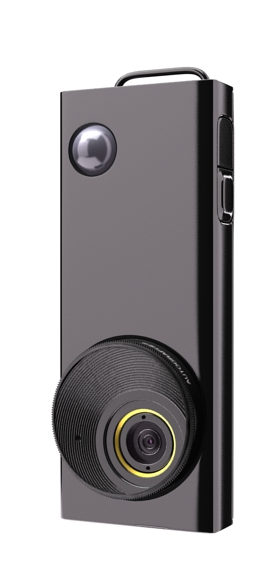
\includegraphics[scale=0.2]{images/Autographer.png} \hspace{25pt}
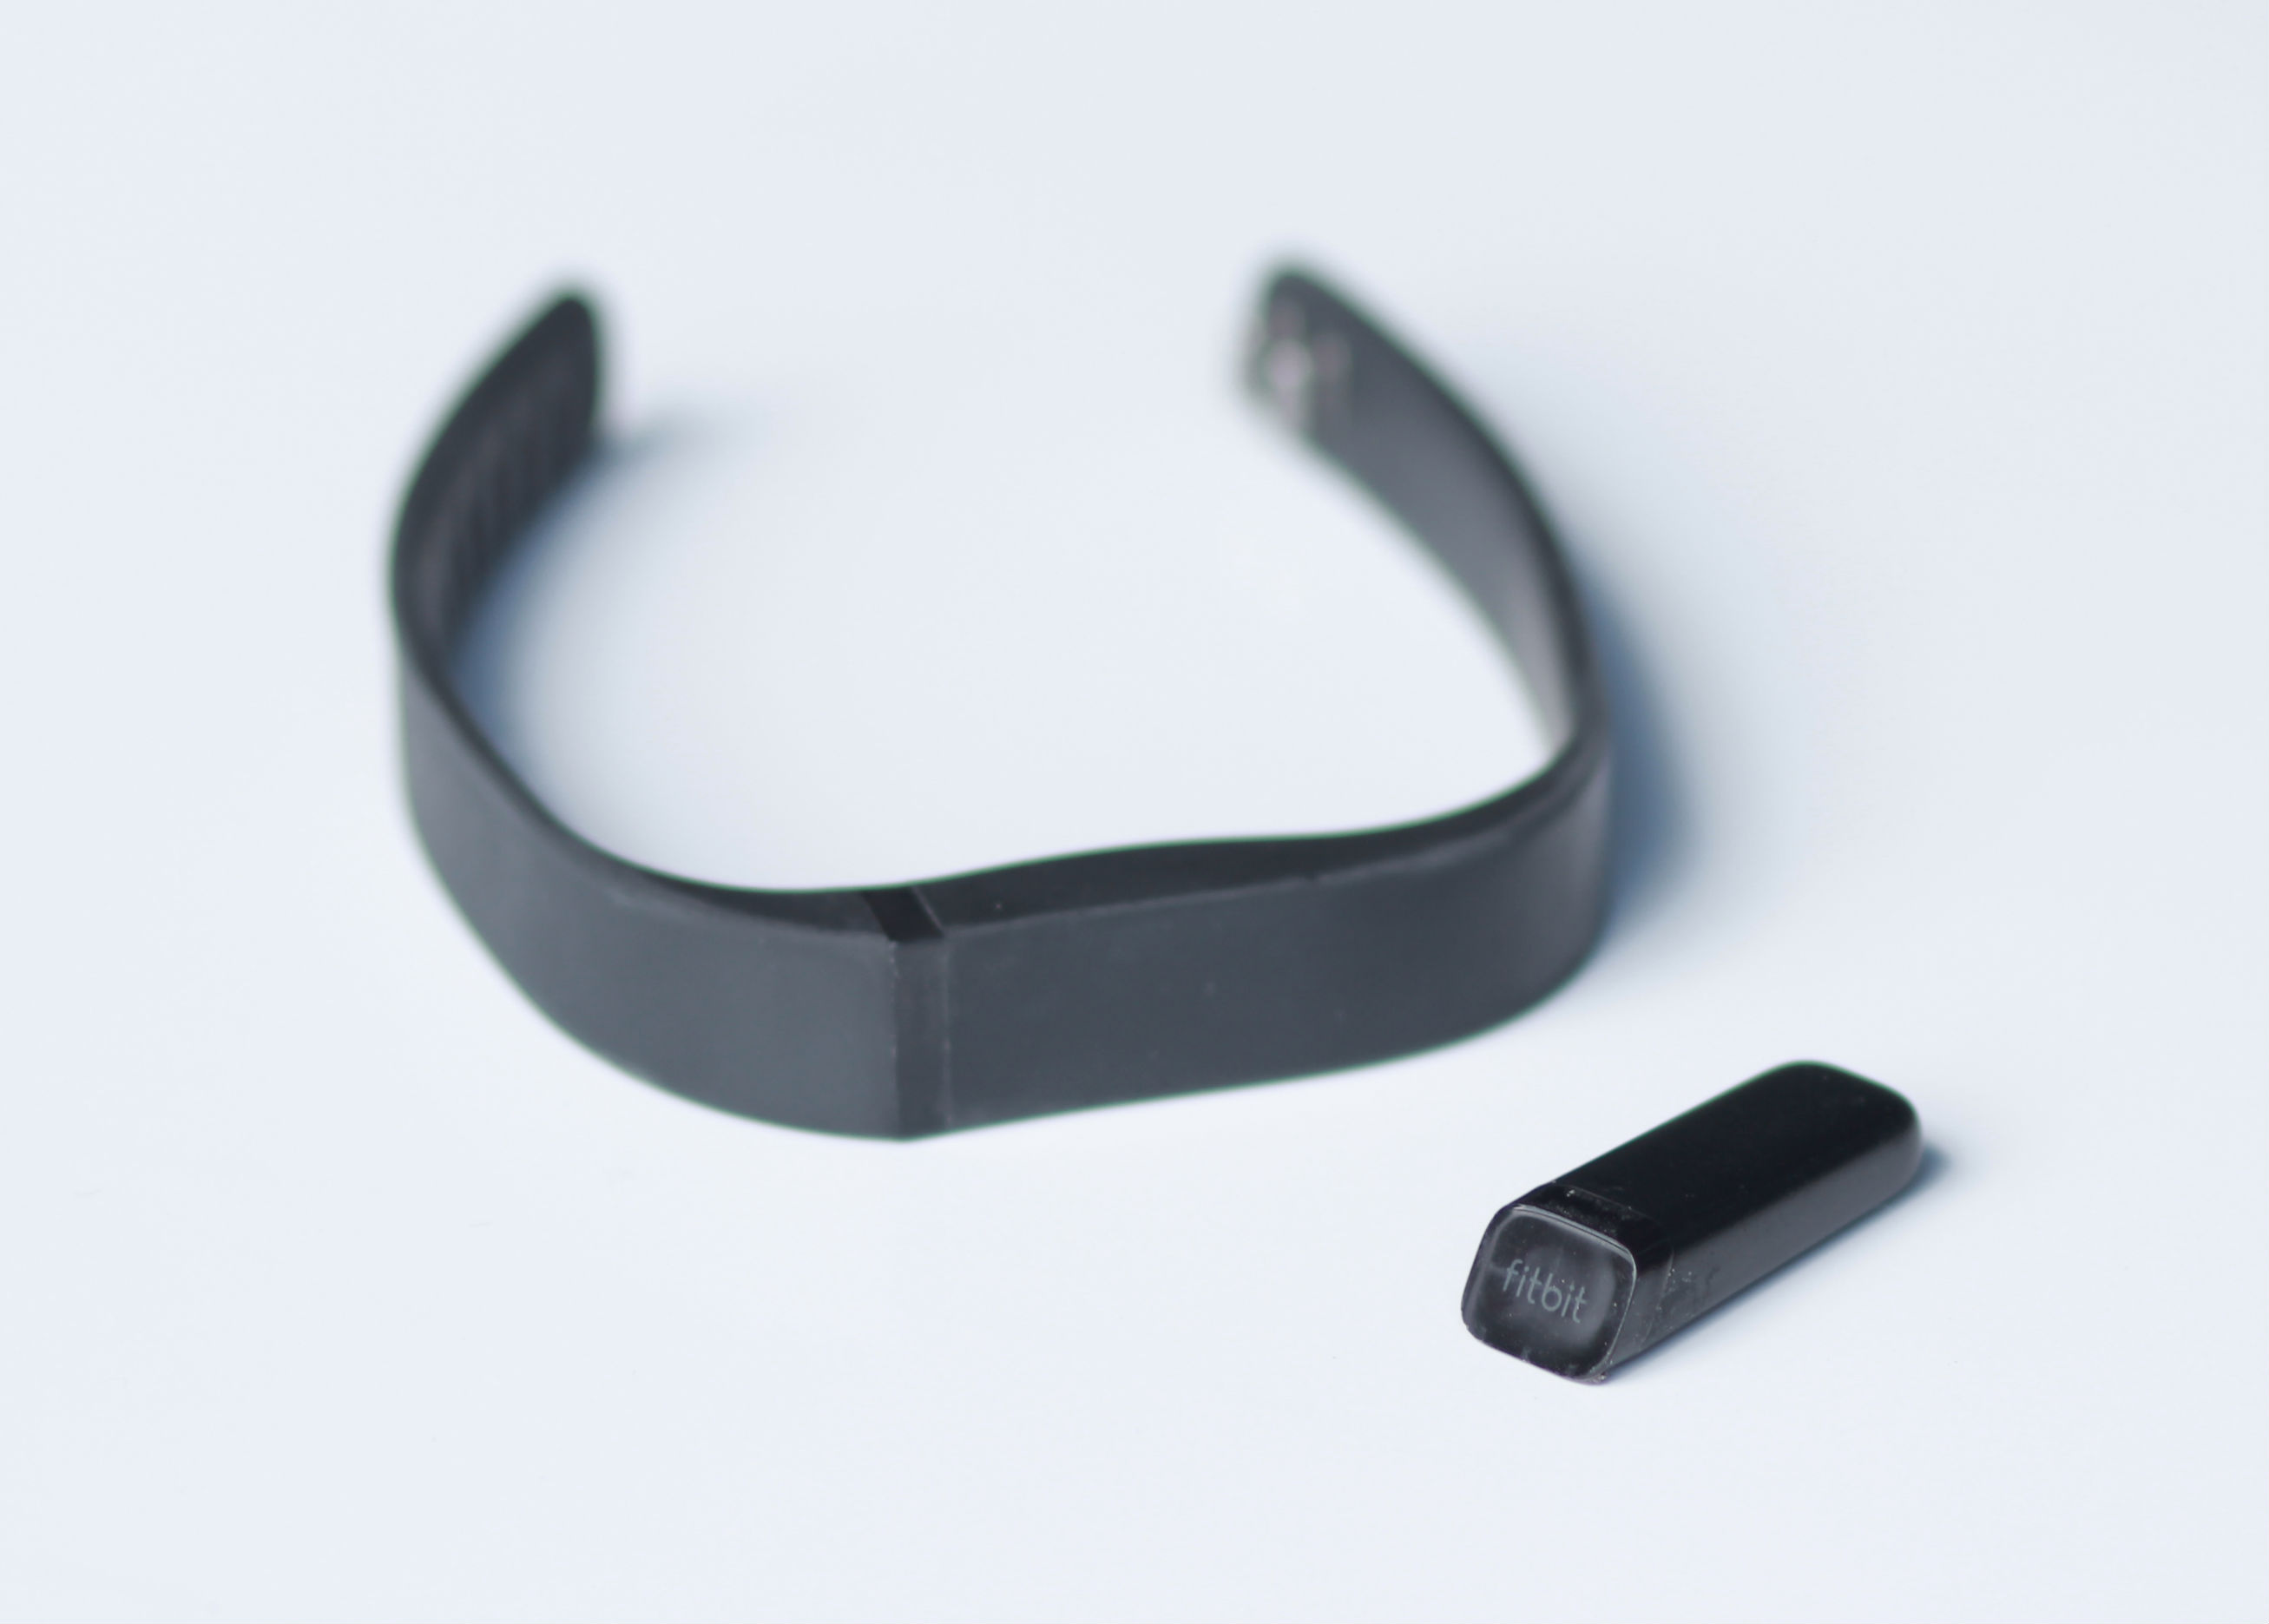
\includegraphics[scale=0.054]{images/Fitibit_Flex.jpg}
\caption{Left: Autographer passive photograph sensor (from \url{https://commons.wikimedia.org/wiki/File:Autographer.png}).\\ Right: Quantified self Fitbit device (from \url{https://commons.wikimedia.org/wiki/File:Fitibit_Flex.jpg}).} \label{fig:test}
\end{figure}

Lifelogging technology encapsulates a range of existing and brand new sensory devices such as audio and visual recording devices, location tracking devices and quantified-self devices. This project as a whole focuses primarily on the way lifelogging data is annotated, how those annotations are evaluated, and the quality of the annotations with respect to a search task. Image annotations are one way of facilitating information retrieval on images. It enables images to be treated like documents such that traditional text-based search models can be applied. This, in combination with the meta data associated with lifelogging images, provides more information about an image than the raw pixel data.

The major challenge that arises with lifelogging is the problem of searching through these vast collections of images. This review will cover literature which has attempted to tackle the problems of representing and indexing vast collections of images, identifying effective annotation models and evaluating these annotations, and finding novel ways to search lifelog data.

In order to create a model of retrieval, there must be some way of structuring the vast collection of data accumulated. The most common and well suited approach, as mentioned by Gurrin et al.~\cite{gurrin2014lifelogging}, is to create a model which mimics the human episodic memory model.

\section{Representing the Data Through Modelling Human Memory}

One way of viewing lifelogging is the process of creating a surrogate memory for a person. Organising and presenting are the key challenges for lifelog search engines. Gurrin et al.~\cite{gurrin2014lifelogging} proposes that it is possible to segment the raw, unprocessed lifelog data into meaningful units, or events; which he defines as: "a temporally related sequence of lifelog data over a period of time with a defined beginning and end". In order to perform information retrieval, the events need to be annotated with meaningful semantics. Annotations can either be manually created by humans, or generated through machine learning algorithms. These annotations must also be evaluated for effectiveness, as poor annotations will lead to poor performance when performing retrieval on the images.

There are five aspects of human memory access, as proposed by Gurrin et al.~\citep{gurrin2014lifelogging}:
\begin{enumerate}
    \item Recollecting: Concerned with re-living and accessing past experiences of episodic memories.
    \item Reminiscing: A form of recollecting, concerned with reliving past experiences for emotional or sentimental reasons.
    \item Retrieving: A more specific form of recollecting  in which specific information needs are to be retrieved such as an address, a document, a location, or any atomic piece of information.
    \item Reflecting: A form of quantified-self analysis, performed in order to discover knowledge and insights that may not be immediately obvious.
    \item Remembering: Concerned with prospective memory more than episodic memory. A form of planning for future activities or to act as a reminder or prompt for tasks that a person would like to do.
\end{enumerate}
Gurrin et al.~\cite{gurrin2014lifelogging} argues that an information retrieval system targeted at lifelogging should focus on the Five R's as information needs for the user.

In the context of searching images on the web,  L. Vuurpij, et al.~\cite{vuurpij2002vind} states that image retrieval systems are restricted to the domain they cover and require a lot of domain knowledge in order to fulfill the information needs of a user. Furthermore, L. Vuurpij, et al.~\cite{vuurpij2002vind} notes that there has been a shift from computer vision and pattern recognition to psychology and cognitive science in the domain of image retrieval, where models like the Five R's~\cite{gurrin2014lifelogging}, are becoming more prevalent. 

\section{Annotating Lifelog Images}
The current state of the art models for image retrieval use tag-based or textual description annotations \citep{ali2010semantically}. This is typically due to the fact that retrieval models can use this text as a bag of words, or to attribute some form of semantic meaning by analysing some text.

\subsection{Types of Annotations}

As suggested by R. Yan et al.~\cite{yan2008learning}, the most common image annotation approaches can be categorised into two types. The first is \textit{tagging}, where annotators choose a set of keywords from a vocabulary for each image. The second most common approach is described as \textit{browsing}, where a group of images are judged against the relevance of a predefined keyword. There are, however, less commonly used annotation approaches, for example, \textit{descriptive natural language annotations} which are generated in a model by A. Karpathy et al.~\cite{karpathy2015deep}. This model outperforms the previous work done in this area of research for both image retrieval and image annotation on the Flickr8K, Flickr300K and MSCOCO. B. Hu et al.~\cite{hu2003ontology} clarifies why high quality textual descriptions generally perform better than systems that employ keyword or tag based annotation models, in that these models suffer from several limitations:
\begin{enumerate}
    \item A keyword in a document does not necessarily mean that the document is relevant
    \item A relevant document may not contain the explicit word
    \item Synonyms of the query keywords lower the recall rate (ratio of retrieved images which are relevant to the total number of relevant images, see Appendix A for details)
    \item Homonyms of the query keywords lower the precision rate  (ratio of relevant images that are successfully retrieved to the total number of relevant and irrelevant images retrieved) see Appendix A for details)
    \item Semantic relations such as hyponymy, meronymy, antonymy are not exploited
\end{enumerate}

Recent work in the consumer health search domain by Zuccon et al.~\cite{quteprints82599} and Stanton et al.~\cite{stanton2014circumlocution} focused on generating queries from images. The aim of their research was to understand how the general public would search for information if they had a medical condition as that in the image presented to them. This new methodology used by these previous works could be adapted to the context of gathering annotations for lifelogging, thus leading to an \textit{annotation by querying} method. This method would consist of showing annotators an image from a lifelogger and ask them to provide the queries they would issue to a (standard) search engine to attempt to retrieve the image itself.
\subsection{Evaluating Annotations}

Without high quality annotations, semantic search would not work, since semantic search exploits the meaning and context of a sentence rather than the keywords in it \cite{ali2010semantically}. The semantic and contextual data associated with images is important for an effective retrieval model that uses textual features rather than pixel data in images. This textual data can either be generated using machine learning algorithms, as demonstrated by A. Karpathy et al.~\cite{karpathy2015deep} and  I. Sutskeve et al.~\cite{sutskever2011generating}, or generated manually by humans. The machine learning algorithms do however start from test data, typically of a specific domain or a range of domains, which they learn from. It is important to note that this can have undesirable consequences when trying to apply a model which has been trained on one domain to one which it has no knowledge of. In both situations, it is essential that the annotations themselves are evaluated such that they describe the image with enough detail and are convincing to humans, since queries will be formulated by humans. Three widely used models for this exist: BLEU \citep{papineni2002bleu} which is precision based, ROUGE (Recall-Oriented Understudy for Gisting Evaluation) \citep{lin2004rouge} which is recall based, and METEOR \citep{elliott2013image}, used for judging the overall quality of annotations.

All of the metrics above were initially proposed with respect to the evaluation of automatic summarisation and natural language processing. Furthermore, they all use a reference annotation in order to score annotations. ROUGE compares the number of overlapping n-grams, word sequences, and word pairs of annotations with ideal annotations created by humans \citep{lin2004rouge}. BLEU counts the maximum number of times a word appears in any reference annotation, followed by "clipping" the total count of each candidate word by its maximum reference count, adding these "clips" up, and dividing by the total unclipped number of candidate words in the annotation \citep{papineni2002bleu}. The notion of "clipping" in BLEU is a variation of precision whereby words are only accepted for the maximum number of times they appear the reference text, for instance if a word appears in an annotation five times but is in the reference annotation twice, the "clipped" value would be 2/5. Finally, METEOR generally operates by unigram matching (bag of words) between a reference annotation, typically created by a machine, and a human produced annotation. Both METEOR and ROUGE take multiple approaches to comparing annotations, for reference, ROUGE:
\begin{enumerate}
    \item ROUGE-N N-gram Co-occurence Statistics
    \item ROUGE-L Longest Common Subsequence
    \item ROUGE-W Weighted Longest Common Subsequence
    \item ROUGE-S Skip-Bigram Co-Occurence Statistics
    \item ROUGE-SU Skip-Bigram Co-Occurence Statistics with Unigram Counting Unit
\end{enumerate}
The unigrams matched in METEOR can be based on surface forms, stemmed forms, and meanings, with the option to be extended \citep{elliott2013image}.

R. Vedantam et al.~\citep{vedantam2015cider} argue through the results of their experimentation, however, that there exists a more effective model for evaluation which is rooted in human consensus. Their method, CIDEr (Concensus-based Image Description Evalutation) is a model which outperforms all other models of evaluating descriptive annotations of images. CIDEr performs so well due to high correlation with human judgement and consensus. According to R. Vedantam et al.~\cite{vedantam2015cider}, the CIDEr metric inherently captures sentence similarity, the notions of grammatically, salience, importance (precision), and accuracy (recall). CIDEr appears to improve upon the other three models and takes into account the weaknesses the other models may have, however it still relies on reference annotations.

The evaluation methods above rely on the availability of a ground truth or reference annotation that can be used to compare with the automatically generated annotation. This approach, however, is ill-suited to generating annotations for lifelog images as it is unclear what these annotations should ``look like'', because it is unknown what makes an annotation of a lifelog image a good annotation. A better suited alternative for this problem is to embed the evaluation of different lifelog annotation methods within a task and thus evaluate the annotation methods with respect to the different effectiveness the different methods induce on the task. Specifically, in this research project, the aim is to embed the evaluation of lifelog annotation within a search task. Thus the effectiveness of a system would be evaluated with respect to the search task. None of the system properties would vary apart from the method that is used to annotate images.~\cite{wei2006lda,zuccon2015integrating,karimzadehgan2010estimation,yi2009comparative}.

\section{Searching for Lifelog Images}

Lifelog information retrieval systems typically have very poor performance due to there not being any formal models made specifically for the field, as reported by Gurrin et al.~\citep{gurrin2014lifelogging}. Until very recently, there have been no large, distributable test collections such as the TREC collection for text \citep{gurrin2014lifelogging}. The NTCIR collection is a set of tagged lifelog images which have been collected by researchers who wore a lifelogging camera for a short amount of time \citep{gurrin2016ntcir}. The tags were automatically generated by using a pre-trained image tagging algorithm.

While there is limited applied methodology to retrieval models in lifelogging, there has been much discussion about what the models should try and solve. Both H.  W.  Bristow et al.~\citep{bristow2004defining} and A. R. Doherty et al.~\cite{doherty2010automatically} corroborate that detecting and interpreting the implicit semantics and context of lifelogging data from heterogeneous sources would be advantageous in explaining the Who?, What?, Where? and When? questions which occur in every day events. It was also noted that these questions are common among image searchers and that they are not capable of being answered by normal indexing like that in traditional search engines \citep{ali2010semantically}.

While there has been some research into tagging and annotating images, there has not been as much work in developing a model for searching these images within the context of lifelogging \citep{gurrin2014lifelogging}. Typical image search engines for web pages treat the surrounding text, captions, alternate text and HTML titles \citep{frankel1996webseer} as a bag of words for retrieval. The success of these search engines rely on a sufficient amount of surrounding text, something which is not provided by current automatic image annotation models for lifelogging. The longer and more detailed the text is within the context of the image, the better the performance of the search engine. This is perhaps why other research has involved novel search techniques \citep{vuurpij2002vind}, since the current models for generating captions of images are not yet detailed or accurate enough for current textual information retrieval models to work.

\section{Conclusion}

Information retrieval for lifelogging is not a narrow subject, but a wide range of domain specific knowledge and fields. From annotations and feature extraction to data storage and models of retrieval, semantically accessing lifelog data is a large and daunting challenge. Since there have never been any significant efforts made to develop formal models for lifelog retrieval and retrieval efforts on significant lifelog data sets are minimal~\cite{gurrin2014lifelogging}, this is the gap in research this work aims to fill. The intent of the research is to investigate and create novel models for lifelog image retrieval and to create a system for annotation collection and evaluation.

This research will explore the different ways images may be annotated, and investigating ways to collected and evalutate the annotations. The reason that no formal lifelogging information retrieval models exist, and that there has not been significant effort made to develop one, is due to the fact that there isn't a sizeable collection of annotated lifelogging data. This is why this research project will put its entire focus into developing the backbone for other research to take place.

%\bibliographystyle{named}
\bibliographystyle{abbrv}
\bibliography{lit-review}

\section{Appendix A}
Precision is defined as 
\begin{equation}
precision = \frac{| \text{relevant documents}\cap\text{retrieved documents}|}{|\text{retrieved documents}|}
\end{equation} and recall,
\begin{equation}
recall = \frac{| \text{relevant documents}\cap\text{retrieved documents}|}{|\text{relevant documents}|}
\end{equation}

These two formulas help to quantify the effectiveness of the following diagram:
\begin{figure}[H]
    \centering
    \includegraphics[scale=0.7]{images/Retrieval.png}
\end{figure}
\end{document}